\documentclass{standalone}
\usepackage{tikz}
\usetikzlibrary{patterns, positioning}
\usepackage[sfdefault]{ClearSans} %% option 'sfdefault' activates Clear Sans as the default text font
\usepackage[T1]{fontenc}

\begin{document}
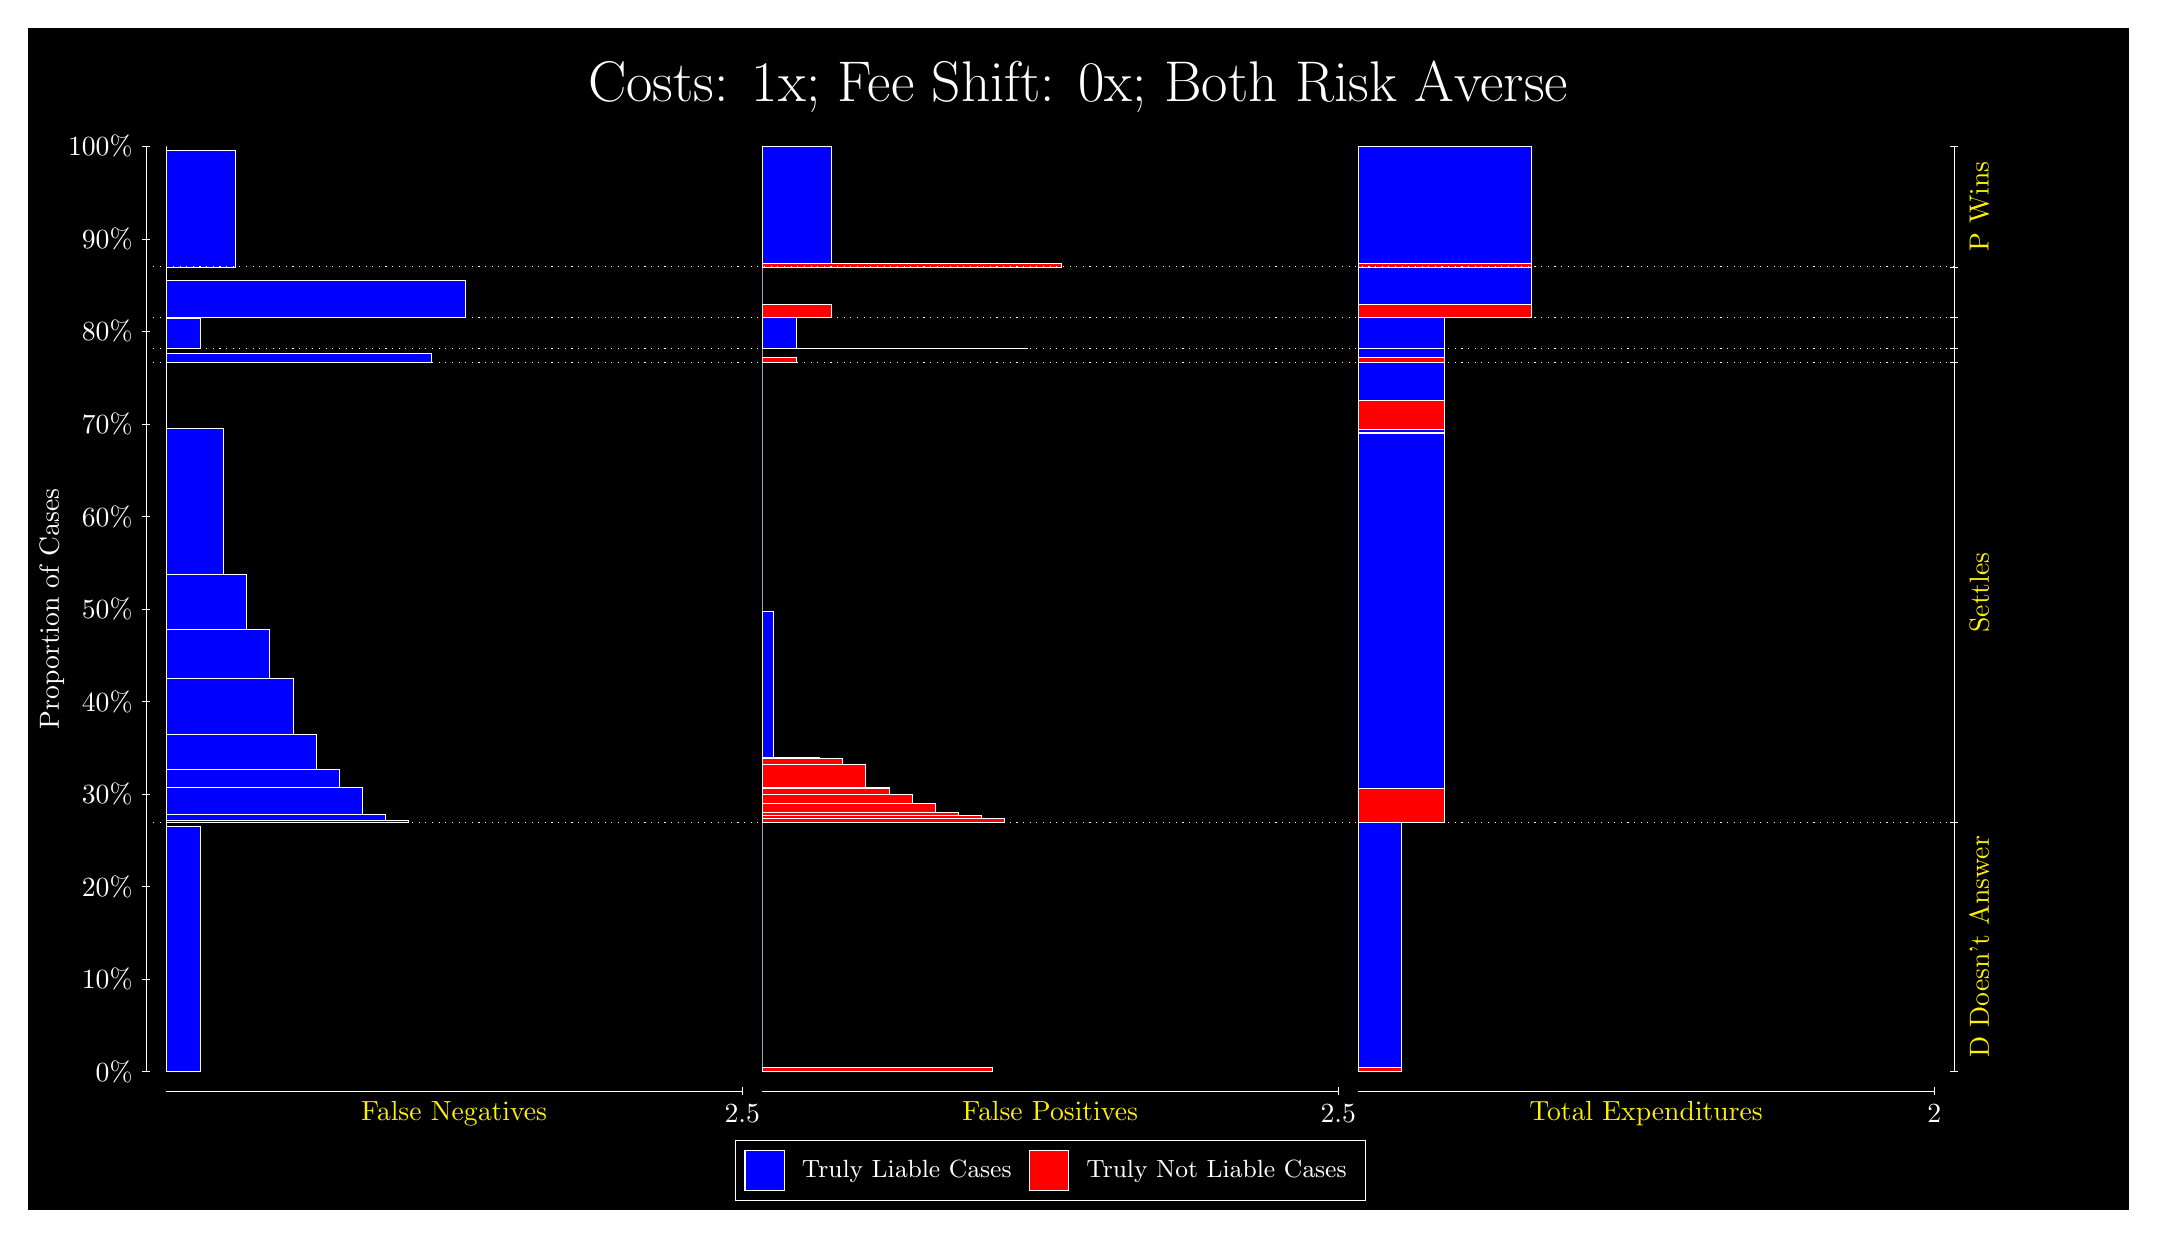
\begin{tikzpicture}
\draw[fill=black] (0,0) rectangle (26.667,15);
\draw[text=white] (0,13.5) rectangle (26.667,15) node[midway] {\huge Costs: 1x; Fee Shift: 0x; Both Risk Averse};
\draw[white, very thin] (1.5,1.75) -- (1.5,13.5);
\node[rotate=90, text=white, anchor=center] at (0.3, 7.625) {Proportion of Cases};
\draw[white, very thin] (1.45,1.75) -- (1.55,1.75);
\node[text=white, anchor=east] at (1.45, 1.75) {0\%};
\draw[white, very thin] (1.45,2.925) -- (1.55,2.925);
\node[text=white, anchor=east] at (1.45, 2.925) {10\%};
\draw[white, very thin] (1.45,4.1) -- (1.55,4.1);
\node[text=white, anchor=east] at (1.45, 4.1) {20\%};
\draw[white, very thin] (1.45,5.275) -- (1.55,5.275);
\node[text=white, anchor=east] at (1.45, 5.275) {30\%};
\draw[white, very thin] (1.45,6.45) -- (1.55,6.45);
\node[text=white, anchor=east] at (1.45, 6.45) {40\%};
\draw[white, very thin] (1.45,7.625) -- (1.55,7.625);
\node[text=white, anchor=east] at (1.45, 7.625) {50\%};
\draw[white, very thin] (1.45,8.8) -- (1.55,8.8);
\node[text=white, anchor=east] at (1.45, 8.8) {60\%};
\draw[white, very thin] (1.45,9.975) -- (1.55,9.975);
\node[text=white, anchor=east] at (1.45, 9.975) {70\%};
\draw[white, very thin] (1.45,11.15) -- (1.55,11.15);
\node[text=white, anchor=east] at (1.45, 11.15) {80\%};
\draw[white, very thin] (1.45,12.325) -- (1.55,12.325);
\node[text=white, anchor=east] at (1.45, 12.325) {90\%};
\draw[white, very thin] (1.45,13.5) -- (1.55,13.5);
\node[text=white, anchor=east] at (1.45, 13.5) {100\%};

\draw[white, very thin] (24.457,1.75) -- (24.457,13.5);
\draw[white, very thin] (24.407,1.75) -- (24.507,1.75);
\node[anchor=west] at (24.407, 1.75) {};
\draw[white, very thin] (24.407,4.9128) -- (24.507,4.9128);
\node[anchor=west] at (24.407, 4.9128) {};
\draw[white, very thin] (24.407,10.753) -- (24.507,10.753);
\node[anchor=west] at (24.407, 10.753) {};
\draw[white, very thin] (24.407,10.934) -- (24.507,10.934);
\node[anchor=west] at (24.407, 10.934) {};
\draw[white, very thin] (24.407,11.328) -- (24.507,11.328);
\node[anchor=west] at (24.407, 11.328) {};
\draw[white, very thin] (24.407,11.969) -- (24.507,11.969);
\node[anchor=west] at (24.407, 11.969) {};
\draw[white, very thin] (24.407,13.5) -- (24.507,13.5);
\node[anchor=west] at (24.407, 13.5) {};

\draw[white, very thin, fill=blue] (1.75,1.75) rectangle (2.1891,4.8639);
\draw[white, very thin, fill=red] (1.75,4.8639) rectangle (1.75,4.9128);
\draw[white, very thin, fill=blue] (1.75,4.9128) rectangle (4.8239,4.9405);
\draw[white, very thin, fill=blue] (1.75,4.9405) rectangle (4.5312,5.011);
\draw[white, very thin, fill=blue] (1.75,5.011) rectangle (4.2384,5.3655);
\draw[white, very thin, fill=blue] (1.75,5.3655) rectangle (3.9457,5.5825);
\draw[white, very thin, fill=blue] (1.75,5.5825) rectangle (3.6529,6.0325);
\draw[white, very thin, fill=blue] (1.75,6.0325) rectangle (3.3602,6.7492);
\draw[white, very thin, fill=blue] (1.75,6.7492) rectangle (3.0674,7.3629);
\draw[white, very thin, fill=blue] (1.75,7.3629) rectangle (2.7746,8.0706);
\draw[white, very thin, fill=blue] (1.75,8.0706) rectangle (2.4819,9.9206);
\draw[white, very thin, fill=red] (1.75,9.9206) rectangle (1.75,10.753);
\draw[white, very thin, fill=blue] (1.75,10.753) rectangle (5.1167,10.872);
\draw[white, very thin, fill=red] (1.75,10.872) rectangle (1.75,10.934);
\draw[white, very thin, fill=blue] (1.75,10.934) rectangle (2.1891,11.321);
\draw[white, very thin, fill=red] (1.75,11.321) rectangle (1.75,11.328);
\draw[white, very thin, fill=blue] (1.75,11.328) rectangle (5.5558,11.797);
\draw[white, very thin, fill=red] (1.75,11.797) rectangle (1.75,11.969);
\draw[white, very thin, fill=blue] (1.75,11.969) rectangle (2.6283,13.448);
\draw[white, very thin, fill=red] (1.75,13.448) rectangle (1.75,13.5);
\draw[white, very thin, fill=red] (9.3189,1.75) rectangle (12.246,1.7989);
\draw[white, very thin, fill=blue] (9.3189,1.7989) rectangle (9.3189,4.9128);
\draw[white, very thin, fill=red] (9.3189,4.9128) rectangle (12.393,4.9691);
\draw[white, very thin, fill=red] (9.3189,4.9691) rectangle (12.1,5.0006);
\draw[white, very thin, fill=red] (9.3189,5.0006) rectangle (11.807,5.0427);
\draw[white, very thin, fill=red] (9.3189,5.0427) rectangle (11.515,5.1625);
\draw[white, very thin, fill=red] (9.3189,5.1625) rectangle (11.222,5.2709);
\draw[white, very thin, fill=red] (9.3189,5.2709) rectangle (10.929,5.3485);
\draw[white, very thin, fill=red] (9.3189,5.3485) rectangle (10.929,5.3656);
\draw[white, very thin, fill=red] (9.3189,5.3656) rectangle (10.636,5.6532);
\draw[white, very thin, fill=red] (9.3189,5.6532) rectangle (10.344,5.7238);
\draw[white, very thin, fill=red] (9.3189,5.7238) rectangle (10.051,5.7454);
\draw[white, very thin, fill=blue] (9.3189,5.7454) rectangle (9.4652,7.5954);
\draw[white, very thin, fill=blue] (9.3189,7.5954) rectangle (9.3189,10.753);
\draw[white, very thin, fill=red] (9.3189,10.753) rectangle (9.758,10.816);
\draw[white, very thin, fill=blue] (9.3189,10.816) rectangle (9.3189,10.934);
\draw[white, very thin, fill=red] (9.3189,10.934) rectangle (12.686,10.941);
\draw[white, very thin, fill=blue] (9.3189,10.941) rectangle (9.758,11.328);
\draw[white, very thin, fill=red] (9.3189,11.328) rectangle (10.197,11.5);
\draw[white, very thin, fill=blue] (9.3189,11.5) rectangle (9.3189,11.969);
\draw[white, very thin, fill=red] (9.3189,11.969) rectangle (13.125,12.021);
\draw[white, very thin, fill=blue] (9.3189,12.021) rectangle (10.197,13.5);
\draw[white, very thin, fill=red] (16.888,1.75) rectangle (17.437,1.7989);
\draw[white, very thin, fill=blue] (16.888,1.7989) rectangle (17.437,4.9128);
\draw[white, very thin, fill=red] (16.888,4.9128) rectangle (17.986,5.3485);
\draw[white, very thin, fill=blue] (16.888,5.3485) rectangle (17.986,9.8519);
\draw[white, very thin, fill=red] (16.888,9.8519) rectangle (17.986,9.8736);
\draw[white, very thin, fill=blue] (16.888,9.8736) rectangle (17.986,9.9013);
\draw[white, very thin, fill=red] (16.888,9.9013) rectangle (17.986,10.277);
\draw[white, very thin, fill=blue] (16.888,10.277) rectangle (17.986,10.753);
\draw[white, very thin, fill=red] (16.888,10.753) rectangle (17.986,10.816);
\draw[white, very thin, fill=blue] (16.888,10.816) rectangle (17.986,10.934);
\draw[white, very thin, fill=red] (16.888,10.934) rectangle (17.986,10.941);
\draw[white, very thin, fill=blue] (16.888,10.941) rectangle (17.986,11.328);
\draw[white, very thin, fill=red] (16.888,11.328) rectangle (19.083,11.5);
\draw[white, very thin, fill=blue] (16.888,11.5) rectangle (19.083,11.969);
\draw[white, very thin, fill=red] (16.888,11.969) rectangle (19.083,12.021);
\draw[white, very thin, fill=blue] (16.888,12.021) rectangle (19.083,13.5);
\draw[white, dotted] (1.5,4.9128) -- (24.457,4.9128);
\draw[white, dotted] (1.5,10.753) -- (24.457,10.753);
\draw[white, dotted] (1.5,10.934) -- (24.457,10.934);
\draw[white, dotted] (1.5,11.328) -- (24.457,11.328);
\draw[white, dotted] (1.5,11.969) -- (24.457,11.969);
\draw[white, very thin] (1.75,1.5) -- (9.0689,1.5);
\node[text=yellow, anchor=north] at (5.4094, 1.5) {False Negatives};
\draw[white, very thin] (9.0689,1.45) -- (9.0689,1.55);
\node[text=white, anchor=north] at (9.0689, 1.45) {2.5};

\draw[white, very thin] (9.3189,1.5) -- (16.638,1.5);
\node[text=yellow, anchor=north] at (12.978, 1.5) {False Positives};
\draw[white, very thin] (16.638,1.45) -- (16.638,1.55);
\node[text=white, anchor=north] at (16.638, 1.45) {2.5};

\draw[white, very thin] (16.888,1.5) -- (24.207,1.5);
\node[text=yellow, anchor=north] at (20.547, 1.5) {Total Expenditures};
\draw[white, very thin] (24.207,1.45) -- (24.207,1.55);
\node[text=white, anchor=north] at (24.207, 1.45) {2};

\node[text=yellow, centered, rotate=90] at (24.777, 3.3314) {D Doesn't Answer};
\node[text=yellow, centered, rotate=90] at (24.777, 7.833) {Settles};



\node[text=yellow, centered, rotate=90] at (24.777, 12.734) {P Wins};

\draw (12.978300999999998,1.5) node[draw=none] (baseCoordinate) {};
\begin{scope}[align=center]
        \matrix[scale=0.5, draw=white, below=0.5cm of baseCoordinate, nodes={draw}, column sep=0.1cm]{
            \node[rectangle, draw, minimum width=0.5cm, minimum height=0.5cm, fill=blue] {}; &
            \node[draw=none, font=\small, text=white] (B) {Truly Liable Cases}; &
            \node[rectangle, draw, minimum width=0.5cm, minimum height=0.5cm, fill=red] {}; &
            \node[draw=none, font=\small, text=white] (B) {Truly Not Liable Cases}; \\
            };
\end{scope}

\end{tikzpicture}
\end{document}